%!TEX root = ../Main.tex

\chapter{Rendering Pipeline}
\label{cha:RenderPipeline}
  \todo[inline]
  {
    Possible titles:

    -- Rendering Workflow

    -- Applying the Rendering Pipeline

    -- Rendering in Vulkan

    -- Rendering Commands and Resource Handling/Management
  }

  \todo[inline]{Pipeline creation? caching?}
  \todo[inline]{Command buffer building. (CBs can be viewed as functions).}
  \todo[inline]{Communication with the GPU}
  \todo[inline]{Image tiling and layout}
  \todo[inline]{Resource transformations.}
  \todo[inline]{Command buffer submission. Mention out-of-order execution. Analogous to CPU instruction dispatch.}
  \todo[inline]{Command buffers can be built once and submitted multiple times. Better performance because no upload (and other things).}
  \todo[inline]{"Setup command buffers", "Draw command buffers", "pre/post-draw command buffers"}
  \todo[inline]{Binding of resource to memory: bind a dummy for as long as the resource loads.}
  \todo[inline]{Diagram for overview of the "pipeline" to give an idea of the whole thing.}

  This chapter describes a set of basic steps to get an image on the screen.
  It assumes a swapchain is set up and ready to be used using the swapchain extension as described in section~\ref{sec:WorkflowAndPatterns}.

  % Command buffers are not unlike procedures where every instruction within that procude is dynamically recorded at runtime.
  % Just like procedures on the \gls{cpu}, command buffers translate to machine instructions on the \gls{gpu}.
  % When a command buffer is submitted, commands within that command buffer may be executed out-of-order, i.e.
  % in another order than they were recorded, if the \gls{driver} or the \gls{gpu} decide to be more efficient in some way.

  % There are two kinds of command buffers: primary command buffers and secondary command buffers.
  % Primary command buffers may be directly submitted to a device queue.
  % Secondary command buffers, on the other hand, must be executed as part of a primary command buffer.
  % The Vulkan command \lstinline{vkCmdExecuteCommands} may be used for this.
  % \todo{Find out more about secondary command buffers!}Secondary command buffers are basically like macros.
  % Secondary command buffers inherit some state form the calling primary command buffer.

  This section will define the framework for the rest of the chapter.
  All examined use-cases of the Vulkan API are moving within this framework.

  \todo[inline]{Vulkan provides many ways to render. In this chapter, one of many ways is explored from beginning to end to show stuff.}

  \todo[inline]{Free moving camera.}
  \todo[inline]{Objects with fixed geometry.}
  \todo[inline]{No complex shading - flat lighting.}
  The graphics scene is kept very simple.
  It only contians objects with fixed geometry.
  The geometry itself may be arbitrarily complex because it has no impact on the usage of the \gls{api}.
  Shaders are also kept simple because this area is not important enough for what is examined in this chapter.

  The shaders used in this chapter are kept very simple.
  Other aspects of Vulkan are more important for this chapter.
  Each object is limited to a single sampled image to be used as a texture.
  As for lighting objects, simple flat shading is performed.
  A vertex consists of the following elements.
  \begin{itemize}
    \item Three \lstinline{float} values representing the position of the vertex in \gls{3d} space.
    \item Two \lstinline{float} values representing the coordinates of the vertex in texture space.
  \end{itemize}

  \todo[inline]{Bring the following into better form.}
  Restrictions:
  \begin{itemize}
    \item Rendering to single window / surface
    \item Forward renderer / single render target
    \item Simple shaders only
    \item Static geometry (no morphing)
    \item Freely moving camera
    \item ...
  \end{itemize}

  \begin{figure}
    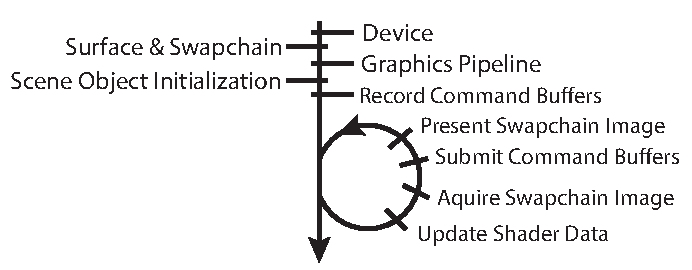
\includegraphics{Main/Images/RenderSetupAndLoopSimple}
    \centering
    \caption{Overview of the setup and execution for a simple forward-render in Vulkan.}
    \label{fig:RenderSetupAndLoopSimple}
  \end{figure}

  \section{Framework}
    \label{sec:Framework}
    \todo[inline]{Explain why this framework is needed. Vulkan offers many possibilities and each application by do things differently.}
    \todo[inline]{Forward renderer.}
    A simple forward renderer is assumed.
    \todo[inline]{Scene with discrete number of objects.}
    The rendered scene will contain a discrete number of objects.
    \todo[inline]{Each object has fixed geometry and a single texture.}
    Each object has fixed geometry and is assigned a single texture.
    \todo[inline]{Single camera that is movable.}
    A camera is used to observe the scene.
    This camera is also movable, e.g. by user-input.
    \todo[inline]{Realtime rendering? Might not be relevant.}
    \todo[inline]{Simple shaders, contents not relevant.}
    Simple shaders are used to render each object of the scene.
    The exact contents of these shaders is not relevant.
    The layout of these shaders is discussed at a later point.

  % \section{Requirements}
  %   Some requirements arise from the framework defined in section~\ref{sec:Framework} which are discussed in this section.
  %   A central requirement is the render target.
  %   Since the ultimate result of a rendering pass is to produce a presentable image, the render target will be an image of the swapchain.
  %   Thus, a swapchain setup as discussed in section~\ref{sec:Pipelines} is required.
  %   In order for each object to be sorted properly during rendering, a depth buffer needs to be set up for the rendering pipeline.

  \section{Setup}
  \label{sec:RenderingSetup}
    \todo[inline]{Before it's possible to render, certain things need to be set up.}
    Before it is possible to start rendering an image, proper Vulkan facilities need to be set up.
    These are discussed in section.
    The setup here adheres to the framework defined in section~\ref{sec:Framework}.

    \subsection{Creating a Proper Device}
      The Vulkan device that is to be used for rendering needs to support both the swapchain extension and queues with graphics and present capabilities.

      In order for a rendered image to be presented to a window, the swapchain extension\footnote{Full name: \lstinline{VK_KHR_swapchain}} needs to be activated.
      This can be done when creating the device.
      Without this extension, no swapchain can be created for this device, which is necessary to present a rendered image in Vulkan.
      Note, however, that the swapchain is not created at this point.
      This has to be done explicitly by the application and is explained later.

      In Vulkan, rendering commands are submitted to a device queue.
      For the purposes of this chapter, queues with two specific capabilities are required.
      These capabilities are called the \textit{graphics capability} and the \textit{present capability}.
      \todo{Is it important \textbf{how} to get the info about the capabilities?}The first specifies whether the queue supports graphics commands such as \lstinline{vkCmdDraw}.
      The second capability specifies whether \lstinline{vkQueuePresentKHR} is supported on that queue.
      Without both of these capabilities, rendering and presenting an image is not possible.
      \todo{Rephrase}A queue might support both of these capabilities but it is also possible that two separate queues are used for graphics and presenting, respectively.
      Once proper queues have been chosen, a logical device can be created.
      This logical device will be used for all subsequent Vulkan operations.
      The queues that were created along with the logical device will be used to submit rendering commands to the \gls{gpu} and to trigger the presentation engine.

    \subsection{Creating a Surface and a Swapchain}
      \todo[inline]{Setup of OS specific surface and swapchain.}
      Now that a device with the enabled swapchain extension is in place, a swapchain can actually be created.
      Creating a swapchain requires what is called a Vulkan \textit{surface} to be created first.
      This surface is operating specific and represents the connection to the actual window.
      It is also the target of the presentation engine, i.e. that surface is used to present a rendered image.

      \todo[inline]{Number, format, extent, colorspace of swapchain images.}
      \todo[inline]{Present modes / VSync.}
      A swapchain consists of multiple images.
      These images are managed by the presentation engine.
      The application may require the swapchain to create a certain number of images constrained to a range defined by the surface.

      \todo[inline]{Move this either to chapter 2 or 3. In this chapter, we mainly care about setting up the swapchain for the framework defined above.}
      The reason why an application may care about the number of swapchain images is rather straight-forward.
      A swapchain image passes some stages until is presented eventually.
      Initially the image is free and can be acquired by the application.
      Once an application acquires the image it is considered to be in use by the application and no longer free.
      At some point, the application hands back the image to the presentation engine, requesting that image to be presented.
      \todo{Explain more presentation modes?}In the \gls{fifo} presentation mode, the image will be put into a queue to be processed by the presentation engine at a convenient time.
      Once that time has come, the image will actually be presented on the surface.
      While an image is either currently presented or still pending presentation in the queue, it cannot be acquired by the application for rendering.
      When there is no free swapchain image, and the application tries to acquire one, the application will be stalled until a swapchain image is available.
      Depending on the chosen presentation mode, the number of swapchain images can be tuned to find the balance that works best for the application.
      Using too many swapchain images wastes memory but not having enough images may stall the application.

      \todo[inline]{Transform mode? Not really relevant for this chapter, right?}
      \todo[inline]{Usage? Swapchain images can always be used as color attachment.}
      Swapchain images will be used exclusively as color attachments for the framebuffer.

    \subsection{Creating a Graphics Pipeline}
      \todo[inline]{Create depth buffer}
      A depth buffer also needs to be created and used within the render pass in order for the objects to be rendered correctly according to how they are ordered.

      \todo[inline]{Create framebuffer for each swapchain image, a render pass, and graphics pipeline. }
      \tbd

    \subsection{Creating Scene Objects}
      \todo[inline]{Create renderable objects. Needs sampled image, geometry. Mention push constants.}
      \tbd

  \section{Command Buffer Recording}
  \label{sec:BuildCommandBuffers}
    \todo[inline]{Mention that this is done on a single thread.}
    \todo[inline]{Mention that this may be done once or multiple times, depending on use of push constants and other things.}
    \todo[inline]{Build command buffers that will never change. Depend on whether push constants are used or not.}
    \todo[inline]{Image layout transition with barriers.}

  \section{Rendering Loop}
  \label{sec:RenderLoop}
    \todo[inline]{Rather simple because of pre-recording command buffers.}
    \todo[inline]{Update uniform buffers.}
    \todo[inline]{Possibly explain push constants.}
    \todo[inline]{Acquire swapchain image.}
    \todo[inline]{Submit command buffers.}
    \todo[inline]{Present swapchain image.}
    \todo[inline]{Sync for submission and presenting (render semaphore, present semaphore) so swapchain image isn't used for rendering while presenting and vice versa. Also image layout transition happens with commands, meaning sync is necessary!}
    \tbd

  \section{Window Resizing}
    \todo[inline]{Should I actually add this section? (Only if there's enough time.)}
    \tbd

  \section{Multi-threaded Rendering}
  \label{sec:MultithreadedRendering}
    \todo[inline]{Introduction to this chapter. Motivation. Additional complexity. Applications must be sure they gain anything from using multi-threading.}
    As mentioned in chapter~\ref{cha:VulkanOverview}, the \gls{driver} has only limited support for multi-threaded access.
    However, this does not mean that multi-threading on the \gls{cpu} has not been taken into account when Vulkan was designed.
    There are actually several ways of utilizing multiple threads for rendering with Vulkan.
    Creating resources and recording command buffers from multiple threads are explored in the following subsections.

    \subsection{Multi-threaded Command Buffer Recording}
      A naive approach to utilize multi-threading is to create several command buffers and assign them to multiple threads.
      These threads would then record commands to their assigned command buffers and submit them to a device queue.
      Unfortunately, there are some problems with this approach.
      According to sections~5.3~and~5.4 of the Vulkan specification\cite{vkspec}, the host application is responsible for synchronizing interactions with command buffers and submitting them to device queues.

      % Problem with command buffers and multi-threaded access.
      Command buffer access is not thread-safe.
      This is because memory used by command buffers is managed by the parent command pool.
      The actual algorithms used for managing memory are left to the \gls{driver}.
      % Done for implementations to be more memory efficient.
      This allows command pools efficient handling of memory operations performed by multiple command buffers, e.g. by allocating more memory than is currently needed and reassigning it as more is requested.
      % Command buffers work on memory managed by parent command pool.
      Because command pools are free to manage memory as they see fit, any operation on a command buffer may trigger side-effects that affect other command buffers created from the same pool.
      This fact alone makes command buffers unsuitable to be shared across multiple threads without synchronization.

      % Command pools do not depend on anything else.
      Command pools, on the other hand, are independent objects.
      The memory they manage is only used for command buffers they created.
      Whenever available memory is no longer sufficient, new memory from the host is requested, optionally using a application-supplied allocator.
      This allocator needs to synchronize low-level allocations, like the C standard library function \lstinline{malloc} already does.
      % Thus solution is to assign each thread its own command pool.
      Synchronization of low-level memory allocation is certainly not as costly as synchronizing each command buffer access.
      Typically, those low-level memory allocations do not happen very often.
      It is likely that command pool implementations strive for minimal host allocations.

      Command pools effectively do not need to be manually synchronized across multiple threads if they are not shared between them.
      In addition, command buffers created from such command pools inherit the same properties.
      Thus, it is more suitable to assign one or more command pools per thread.
      % Threads then allocate and record into as many command buffers as needed.
      Each thread is then free to allocate and record into as many command buffers as needed without having to conduct fine-grained synchronization.

      % Let main thread submit command buffers by sharing a datastructure with synchronized access.
      In order for command buffers allocated on other threads to be submitted to the device queue, the main thread may provide a shared datastructure that is capable of containing command buffer objects.
      Access to this shared container would be synchronized using traditional synchronization methods.
      % Turns the initial problem into well-understood producer-consumer problem\cite{EWD:EWD329}.
      % Solves the inital queue submission problem.
      This effectively creates the well-understood producer-consumer scenario\cite{EWD:EWD329} and solves the initial queue submission problem.

      \todo[inline]{Prev paragraph is just a suggestion. May be better to do differently. Depends on application.}

      \subsubsection{Command Buffer Management Considerations}
        % ... There is another problem with the system mentioned above.
        % ... It is also recommended to assign more than one command pool to an individual thread.
        % ... While a command buffer is being processed, i.e. once it has been submitted but has not finished execution yet, the command buffer should not be modified.
        % ... The reason why multiple pools should be used instead of simply creating new command buffers from the same pool is because of the underlying memory model.

        % ... In the previously described scenario, each thread has exactly one command pool that is used to create multiple command buffers from.
        % ... Commands are recorded to these command buffers and are submitted in batches to the device for execution.
        % ... Vulkan specifies some restrictions on what may be done with command buffers that are pending execution.
        % ... For example, the application should not free a command buffer that is pending execution.

        % Command buffers need to be kept alive while pending execution.
        Vulkan prohibits modifying submitted command buffers that are pending execution on the device.
        This includes freeing these command buffers, i.e. the application is responsible for keeping them alive as long as they are pending execution.
        In practice, this effectively means command buffers submitted in batches may only be modified or reused once the entire submission has finished execution because it is hard to predict when individual commands are processed if more than one command buffer is submitted.
        Out-of-order execution is one reason for this unpredictability.
        The simplest way to solve this problem is to just use new command buffers for every new batch submission.
        This poses some management overhead since individual command buffers need to be associated to these batches in some way in order to be freed or reused.
        Vulkan does not do this automatically.
        Otherwise, if command buffers are never freed, the application ends up allocating a lot more than necessary, effectively leaking memory.

        % Command pools better than just using command buffers because of decoupled underlying memory and clean separation of concern.
        A better way might be to use command pools for this purpose.
        Managing command buffers is already what they do and it also offers a clean separation of concerns between the different batches of command buffers.
        In other words, using command pools to allocate command buffers that are submitted together provides a way to manage these command buffers using standard methods.
        Vulkan allows command pools to be reset, effectively resetting all command buffers spawned from them, respectively.
        This means that command pools may be reused after their associated batch of submitted command buffers has finished execution.
        When resetting a command pool, the host application is free to choose whether memory allocated by that command pool should be released or not.
        If a command pool is going to be reused, and the memory is not released, this command pool can directly start producing command buffers without causing additional allocation overhead.
        This provides a clean way for managing command buffer lifetimes without the need to use anything but the Vulkan \gls{api} itself.

        \todo{Describe what they did differently?}Similar approaches have been described by industry experts such as Marius Bjørge\cite{bjorge:multithreadingvulkan} in his blog post about multi-threading in Vulkan as well as Mathias Schott\cite{mschott:vulkan_multi_threading} in his talk entitled "Vulkan multi-threading".

        Care must be taken, however, in cases where the amount of memory required by a command buffer is not steady during its lifetime.
        For example, when transitioning from a large \gls{3d} scene, with many objects to render, to a small scene with less draw calls to perform, the memory requirements of each command buffer may be lowered considerably for the new scene.
        In cases like this, it might make sense to reset all relevant command buffers, freeing their associated memory.
        Switching from a small scene to larger one is not a problem, of course, because the command buffer will simply allocate enough memory for the new scene.


    \subsection{Multi-threaded Resource Creation}
      Vulkan applications need to create resources such as images and shaders.
      Loading and creating these resources may take a considerable amount of time, depending on the data in question.
      Images, for example, can be quite large.
      They may also have to be transformed in some way which also consumes computation time.
      Shaders need to be compiled (by the \gls{driver}) and bound to a Vulkan pipeline.
      Many of these time consuming operations work more or less independently from the rest of the system, depending on the specific operation.
      This makes them interesting candidates for execution on multiple threads.
      However, the use of multi-threaded resource creation introduces additional complexity to the system.

      First of all, an application has to decide how many threads are actually needed for resource creation.
      It is possible that only one dedicated resource creation thread is sufficient for many applications.
      The actual number of resource creation threads depends on the application.

      All resource creation threads need device memory in one way or another.
      There are basically two ways of accomplishing this without race conditions.
      The first way is to preallocate the memory that is available for each thread.
      This method does not require synchronization between threads because each is assigned a memory region that is not overlapping memory from other threads.
      The second way is to assign a memory allocator to each thread that internally synchronizes the calls.
      This method does not require the main thread to know the size of the resources each thread creates but memory allocations need to be synchronized.
      Again, the method of choice depends on the application.
